\documentclass[a4paper, 12pt, french]{report}

\usepackage[utf8]{inputenc} % UTF-8
\usepackage{babel} % French 
\usepackage[T1]{fontenc} % Times New Roman
% \usepackage[latin1]{inputenc} % ISO 8859-1
\usepackage{lmodern} % modern fonts
\usepackage[babel=true]{csquotes} % French quotes
\usepackage{minitoc} % Table of contents
\usepackage{geometry} % Page size
\usepackage{ragged2e} % Ragged right
\usepackage{fancyhdr} % Header
\usepackage{graphicx} % Images
\usepackage[scaled]{helvet} 
\usepackage{listings} % Code
\usepackage{amsthm}
\usepackage{tabularx}
% \usepackage{hyperref}
\usepackage[hidelinks]{hyperref}
% \usepackage{minted}
% \usepackage{glossaries}

\newtheorem{definition}{Définition}

\graphicspath{ {./src/images/} }

\justifying
\setlength{\headheight}{0.5cm}
\setlength{\headsep}{0.5cm}

\renewcommand{\baselinestretch}{1.5}

\geometry{hmargin=2.5cm,vmargin=2.5cm}

\setcounter{secnumdepth}{3} % Section number depth
\setcounter{tocdepth}{1} % Table of contents depth
\setcounter{minitocdepth}{3} % Table of contents depth

\begin{document}

% Intro             ===============================
\begin{titlepage}
    \begin{center}
        \vspace*{0.5cm}

        
\includegraphics[scale=0.50]{logo_ufr_sen.png}
        \hspace{2cm}

        \vspace{0.5cm}

        \textbf{\Huge{ISYEB}}

        \vspace{0.5cm}

        \rule{\linewidth}{0.5mm}
        \textbf{Rapport de stage de 3ème année de Licence Informatique} 
        
        \vspace{0.2cm}

        \small{\textit{Sujet : Réalisation d'un dispositif de capture vidéo pour l’acquisition de données dans le cadre d’une manipulation en biologie.}}
        \rule{\linewidth}{0.5mm}

        \vspace{1.5cm}

        \textbf{Nom :} \textit{M. BOULANGER} \\
    
        \textbf{Aymerick LAURETTA-PERONNE} \\

        \vfill
                
		{\large Organisme d'accueil: \textsl{Université des Antilles Département de Biologie}} \\[0.1cm]
        \small{\textit{Équipe Biologie de la Mangrovee}} \\[1.5cm]

		\begin{minipage}{0.7\textwidth}
			\begin{flushleft}
				Enseignant référent: \\
				\hspace{0.2cm} Wilfried \textsc{SEGRETIER}
			\end{flushleft}
		\end{minipage}
        
		\vspace{-0.85cm}
		\hspace{9cm}
		\begin{minipage}{0.3\textwidth}
			\begin{flushleft}
				Tuteur de stage: \\
				\hspace{0.2cm} Manuel \textsc{CLERGUE}

				Co-tuteur: \\
				\hspace{0.2cm} Olivier \textsc{GROS}
			\end{flushleft}
		\end{minipage} \\[3cm]

        \rule{\linewidth}{0.5mm}
        \vfill
        
        \textbf{Université des Antilles} \\
        \textbf{Département de Biologie} \\
        \textbf{Équipe Biologie de la Mangrovee} \\
        \textbf{Laboratoire de Biologie Marine} \\
        \vspace{0.5cm}
        \textbf{\today {}}
         
    \end{center}
\end{titlepage}
% Intro             ===============================

% White Sheet        ===============================
% \newpage
% \thispagestyle{empty}
% \mbox{}
% \newpage
% White Sheet        ===============================

% Remerciments             ===============================
\begin{center}
    \textbf{\large{Remerciments}} \\[2cm]

    Je tiens à remercier tout ceux qui ont contribué à la réalisation de ce rapport de stage. \\[0.5cm]

    Tout d'abod, je tiens exprimé ma gratitude à Monsieur Manuel CLERGUE de m'avoir accepté et accompagné durant mon stage. \\[0.5cm]

    J'adresse mes remerciments à Monsieur Olivier GROS pour l'accueil chaleureuse au sein de l'équipe et de m'avoir fait partager ses connaissances et ses expériences dans le domaine de la biologie. \\[0.5cm]

    Merci à tous les membres de l'équipe de Biologie de la Mangrovee pour leur aide et leur soutien. \\[0.5cm]

    
\end{center}
% Remerciments             ===============================

% Résumé             ===============================
\vspace*{\fill}
    \section*{Résumé}
        Dans ce rapport sont présentées les différentes étapes de conception du dispositif de capture vidéo et de la réalisation de l'application pour les biologistes du laboratoire ISYEB.
        Ce dispositif a pour but de remplacer celui existant du laboratoire ISYEB en offrant une meilleure polyvalence aux biologistes.
        L'application quant à elle doit permettre aux biologistes de réaliser différents types de prises de vue de manière plus efficace et autonome en fonction de leurs besoins.
        De ce fait, l'application doit permettre aux biologistes de lancer un enregistrement en ayant la possibilité de choisir l'emplacement et le nom du fichier vidéo enregistré. Permettre aussi la prise de photo en ayant la possibilité tout comme l'enregistrement vidéo de choisir l'emplacement et le nom du fichier photo enregistré.
        Ce dispositif doit permettre aux biologistes de récupérer les différents enregistrements via a différents types de périphériques externes de stockage en ayant également une possibilité de les visualiser depuis le dispositif.



    \section*{Abstract}
        In this report are presented the different stages of design of the video capture device and the realization of the application for the biologists of the ISYEB laboratory.
        The purpose of this device is to replace the existing one in the ISYEB laboratory by offering better versatility to biologists.
        As for the application, it should enable biologists to take different types of shots more efficiently and autonomously according to their needs.
        Therefore, the application must allow biologists to launch a recording by having the possibility of choosing the location and the name of the recorded video file. Also allow photo taking with the possibility, like video recording, of choosing the location and name of the saved photo file.
        This device must allow biologists to retrieve the different recordings via different types of external storage devices while also having the possibility of viewing them from the device.
\vspace*{\fill}
% Résumé             ===============================

\dominitoc
\tableofcontents


% Introduction             ===============================
\chapter{Introduction}
\minitoc
    
    \section{Présentation}
% Introduction             ===============================

% Environnement             ===============================
\chapter{Environnement}
    \section{L'université des Antilles}
    L’université des Antilles est une université pluridisciplinaire implantée sur deux régions, Guadeloupe et Martinique née de la scission de l’université des Antilles et de la Guyane (UAG) en 2014, en université de Guyane, d’une part et en université des Antilles, d’autre part.

    \vspace{0.5cm}

    Elle comprend l'une des 204 écoles d'ingénieurs françaises accréditées au 1er septembre 2020 à délivrer un diplôme d'ingénieur.

    \section{L'UFR SEN}
    L’Unité de Formation et de Recherche (UFR) en Sciences Exactes et Naturelles (SEN), communément appelée UFR SEN, compte près de 1 800 étudiants, 110 enseignants et enseignants chercheurs, 32 personnels BIATSS, et a la particularité d’être la composante de l’Université des Antilles qui porte le plus de diplômes de formation (15) et de structures de recherche (9 sur les 25 que compte toute l’université). 
    Ses domaines de recherche et de formation couvrent les six pôles thématiques de l’Université des Antilles : Risques et Énergies, Numérique, Mer et Océan, Biodiversité en milieu tropical insulaire, Santé insulaire en environnement tropical, Dynamique des sociétés et territoires Caraïbes.

    \vspace{0.5cm}

    Les équipes de recherche portent à elles seules près de 70\% de l’ensemble des projets de recherche réalisé à l’Université des Antilles.
    Des impacts environnementaux des sargasses, à l’étude de la durabilité des matériaux, en passant par les risques naturels majeurs et les transitions énergétiques, climatiques et écologiques, la Faculté des Sciences est porteuse de projets innovants. 

    % \vspace{1cm}

    \section{L'Equipe de la Biologie de la Mangrove}
    L'équipe \textbf{Biologie de la Mangrove} fait partie intégrante de l'UMR 7205 MNHN CNRS-Sorbonne Université-UA <<Institut de Systématique, Evolution, Biodiversité>> dirigée par \underline{Philippe Grandcolas}.

    \vspace{0.5cm}

    \begin{flushleft}
        Elle représente l'une des 19 équipes constituant actuellement cette UMR qui est répartie sur 2 sites (Paris et Guadeloupe). L'équipe \textbf{Biologie de la Mangrove} est composée exclusivement de personnels de l'Université des Antilles et est localisée en Guadeloupe sur le campus de Fouillole.

        \vspace{0.5cm}
        
        L'équipe de la Biologie de la Mangrove intégré l'UMR 7205 ISYEB en janvier 2019 en proposant d'étudier la biologie et les adaptations évolutives (par le biais de la symbiose essentiellement) de modèles littoraux côtiers tropicaux évoluant au sein d'écosystèmes extrêmes (forte teneurs en composés soufrés réduits comme la mangrove et les herbiers à phanérogames marines) faciles d'accès.
    
        \vspace{0.5cm}
    
        Mon tuteur en entreprise durant le stage est Monsieur \underline{Olivier GROS} responsable de l'équipe Biologie de la Mangrove et Professeur des Universités.
        Les étapes de développement de l'application est validée par Monsieur \underline{Manuel CLERGUE} également Professeur et chercheur à l'Université des Antilles.
        Les membres de l'équipe projet Monsieur \underline{Matheiu BONNEAU} intervenant Mathématique et Madame \underline{SUZANNE} doctorante et la stagiaire en Biologie qui aura la gestion des expériences.

    \end{flushleft}


    \section{Ressources fournies}
    Plusieurs ressources m'ont été fournies dans le cadre de mon stage.
    Dans un premier temps, j'ai reçu le matériel permettant l'acquisition vidéo qui sera abordé dans la section 4.2.
    Une connexion filaire au réseau de l'Université des Antilles a été fournie pour me permettant d'installer des mise à jour de logiciels.

    \section{Organisation du stage}
    Tout au long du stage, des réunions régulières on été organisées avec mon encadrant Monsieur \underline{Manuel CLERGUE} afin de faire le point sur l'avancement du projet.

    \begin{flushleft}
        Le travail a été répartie en deux axes :
        % Première partie en laboratoire
        % Seconde partie sur le terrain 
        \begin{itemize}
            \item  \textbf{Partie en laboratoire}
            \item  \textbf{Partie sur le terrain}
        \end{itemize}
        
        \vspace{0.5cm}      
    \end{flushleft}

    \section{Contraintes particulière}
    Durant ce stage j'ai eu deux contraintes particulières :
    \begin{itemize}
        \item  Premièrement, le matériel ayant été commandé avant le début de mon stage et des différents aspects techniques.
        \item  Deuxièmement, le calendrier stricte en début de stage demandant un système minimal en 10 jours.
    \end{itemize}
% Environnement             ===============================
    
% Présentation de la problématique (sujet du stage)          ===============================
\chapter{Présentation de la problématique}
    \section{Présentation du sujet}
    Projet avec le laboratoire de \textit{Biologie} de l'\textit{Université des Antilles}, le projet concerne en l'analyse de déplacement de \textbf{Gerridés} afin de déterminer leur préférence sur des zones marquées par des odeurs, en environnement contrôlé.

    % \vspace{0.5cm}

    \section{Présentation de l'aspect biologistes}
    Les \textbf{Gerridés} sont une famille d'insectes de l'ordre des Hémiptères et du sous-ordre des Hétéroptères c'est-à-dire des punaises.
    \begin{figure}[ht]
        \centering
        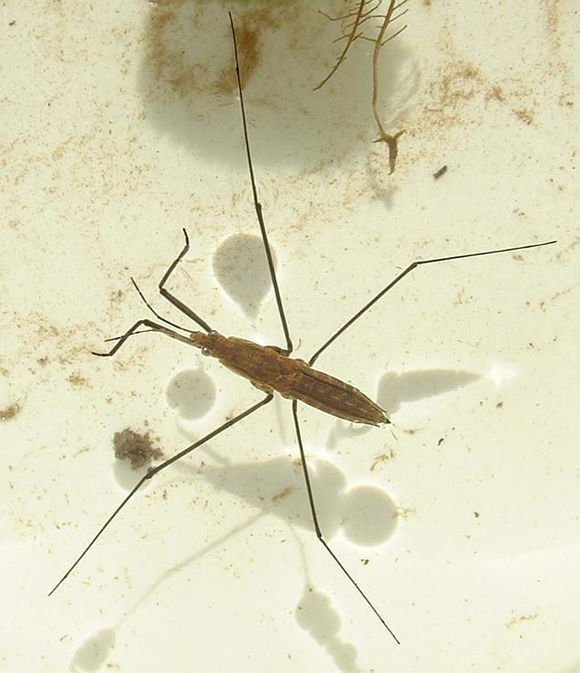
\includegraphics[scale=0.15]{gerrides.jpg}
        \caption{Gérridés}        
    \end{figure}

    \vspace{0.1cm}

    \begin{flushleft}
        Les membres de cette famille sont communément appelés araignées d’eau, mais ce sont des insectes, on ne peut donc pas parler d'araignées. Cette appellation vient sans doute du fait de leurs longues pattes. Leur capacité à se déplacer sur l'eau leur vaut aussi le nom de patineurs de l'eau.\\[0.1cm]
        
        J'ai eu l'occasion de partir à la recherche de Gérridés dans la Mangrove de la Guadeloupe et d'en attraper a l'épuisette (voir Figure 3.2).

        \begin{figure}[ht]
            \centering
            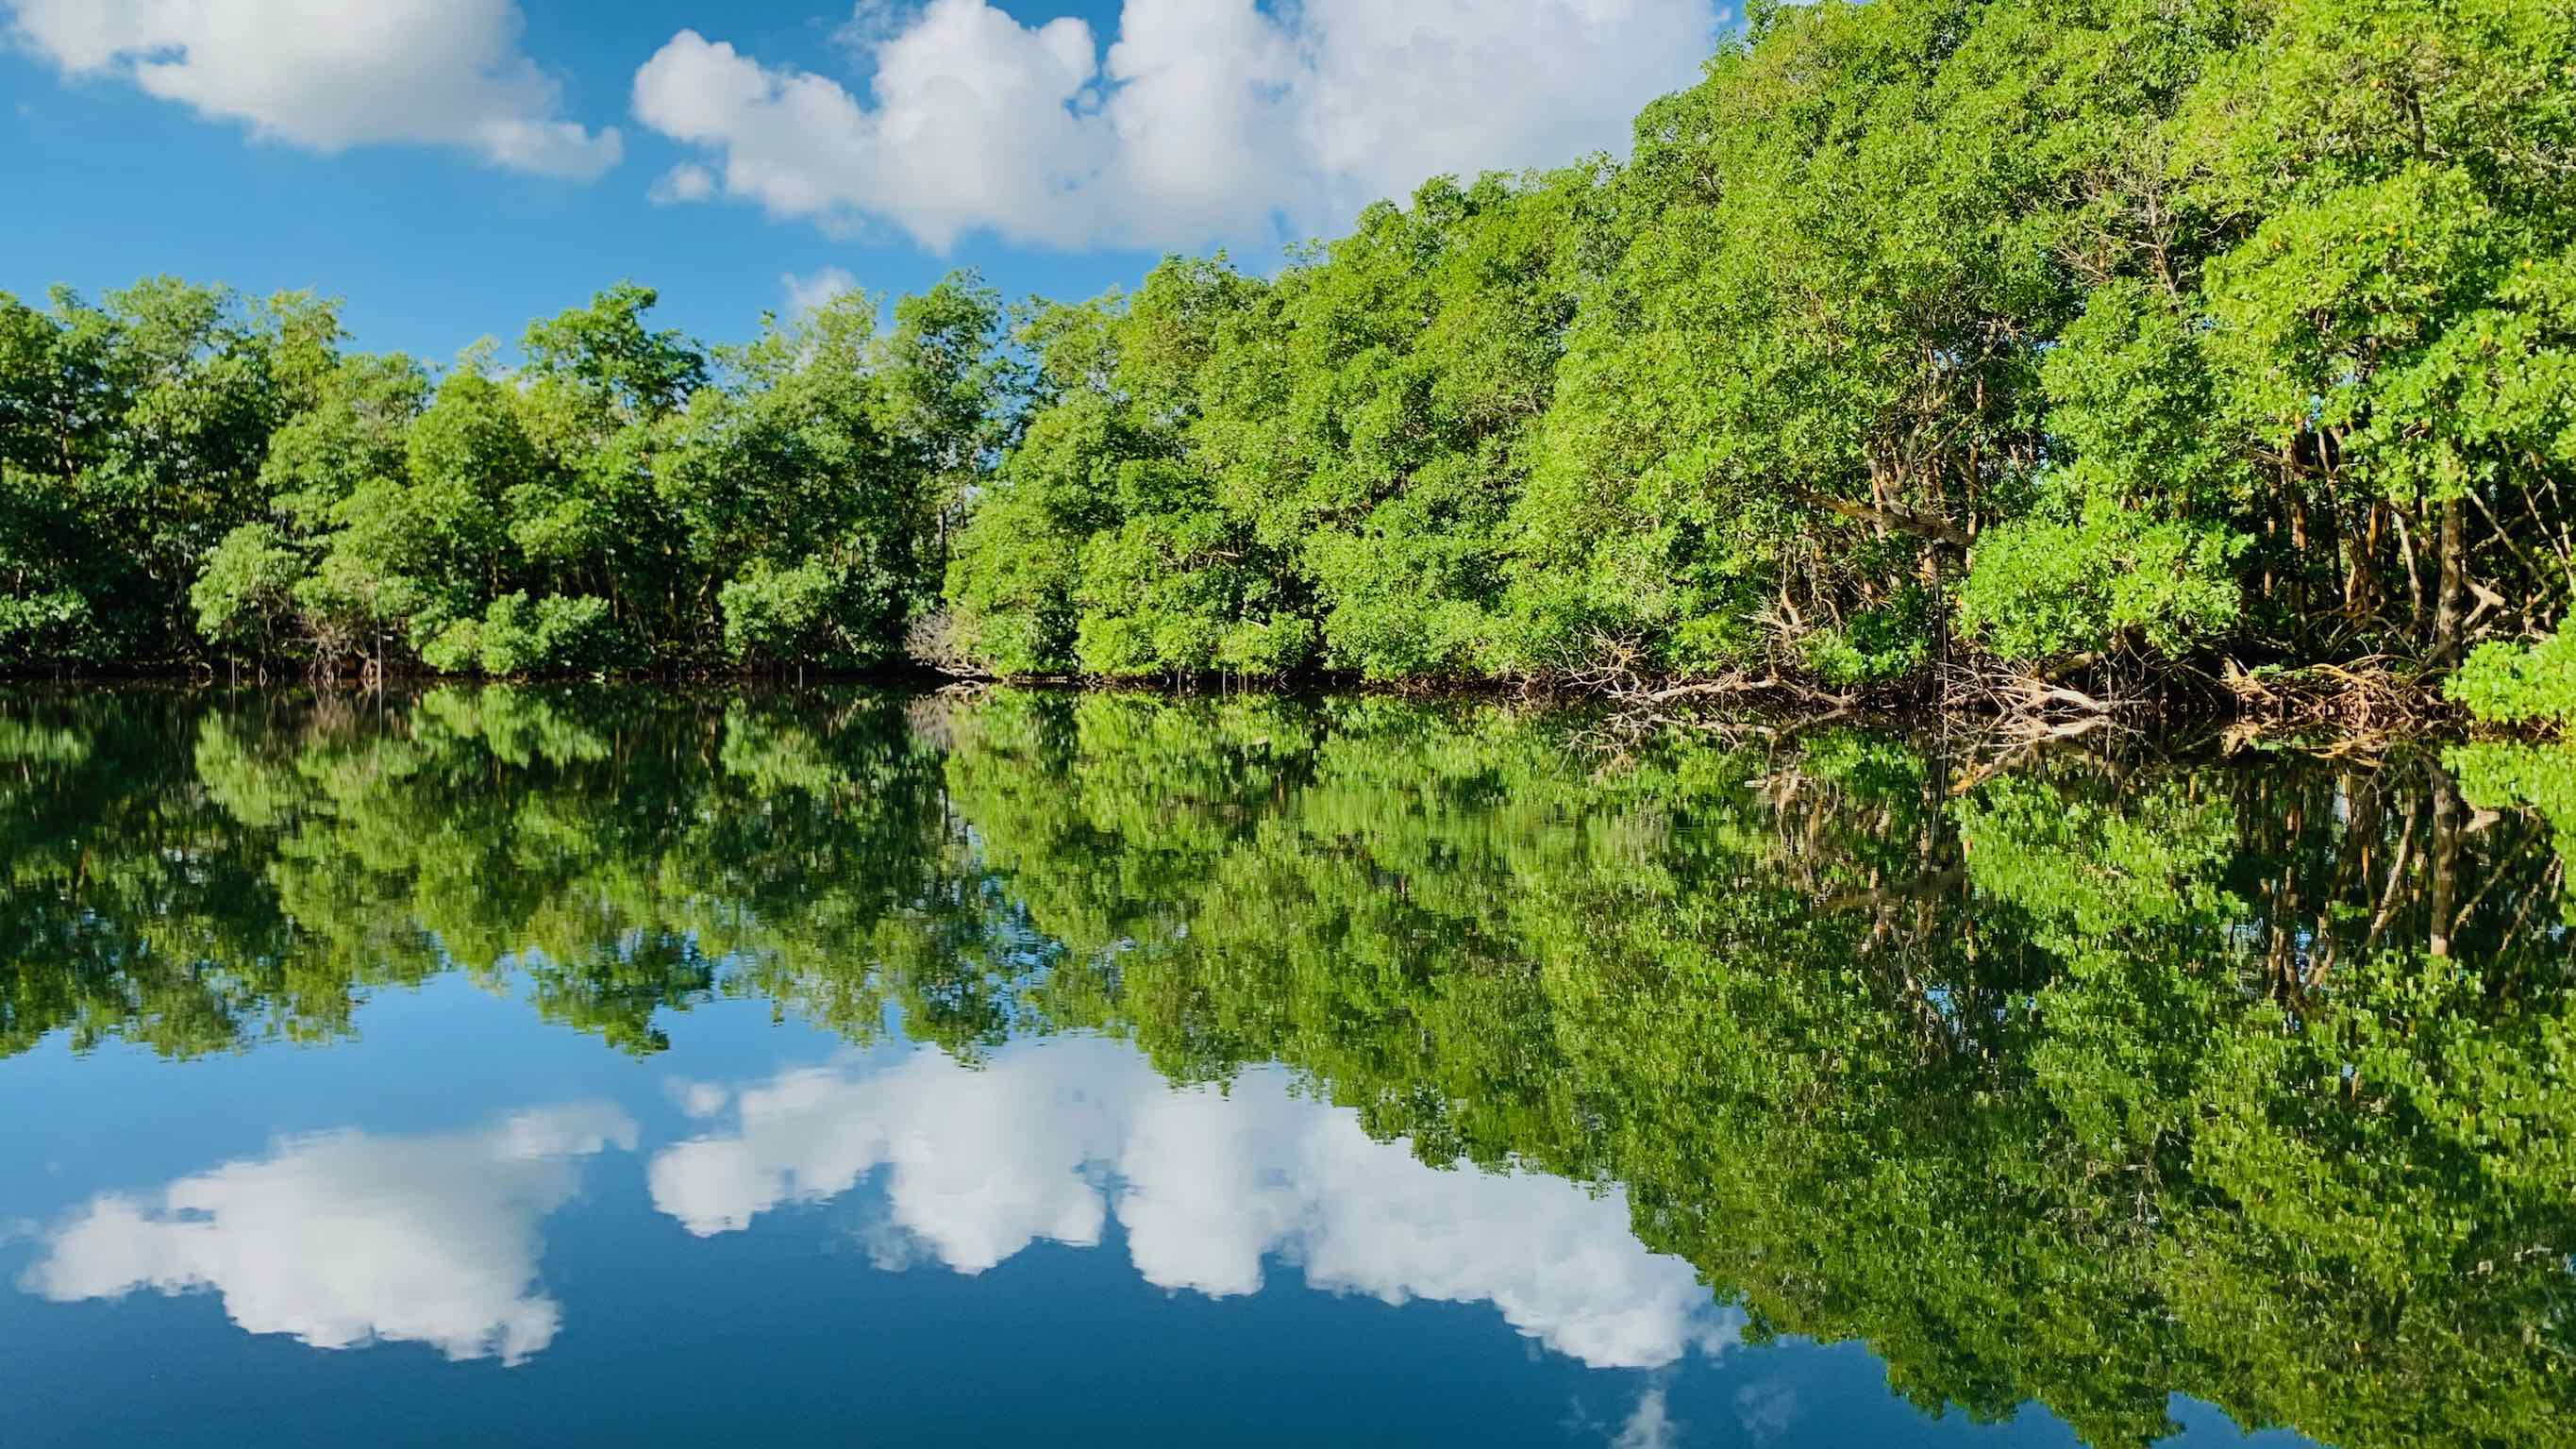
\includegraphics[scale=0.05]{mangrove.jpeg}
            \caption{Mangrove de la Guadeloupe}
        \end{figure}


    \end{flushleft}

    \vspace{0.2cm}

    Afin de déterminer leur préférence, il est nécessaire d'avoir un dispositif adéquat de capture vidéo pour l'acquisition de données.

    \vspace{0.5cm}

    \begin{flushleft}
        Le tout étant fait de façon manuelle, les biologistes accrochaient une GoPro au dessus du bac et ensuite devaient la rettirer afin de pouvoir récupérer les données enregistrées. Ce dispositif était fonctionnel et leur permettait de réaliser des captures vidéo mais ils leur fallait placé le bac dans le champ de vision de la GoPro a chaque fois qu'ils voulaient faire une capture.\\[0.2cm]
        
        Il fallait aussi que la GoPro soit connecté à un ordinateur afin de pouvoir récupérer les données.\\[0.2cm]

        Ajouter à cela le démarrage et l'arrêt de l'enregistrement de manière manuelle entrainant régulièrement le déplacement du bac (avec les mouvements). La disposition de la GoPro ne permettait de bien voir la prévisualisation de la capture vidéo.\\[0.2cm]

        Les biologistes ont donc décidé d'améliorer leur dispositif afin de pouvoir réaliser l'expérience de manière plus pratique.\\[0.2cm]

        Ce qui nous peremets d'enchainer sur l'objectif qui en découlent.

    \end{flushleft}

    \vspace{0.1cm}

    % Pourquoi : Avant c'était fait à la main et c'est pas très efficace.

    \section{Objectifs}
    % Voir pour mettre cette partie dans 'Mon Travail' 4.1.
    L'objectifs du stage est de réaliser l'installation et de configurer un dispositif de capture vidéo réalisé par un \textit{Raspberry Pi} ainsi que de développer une application conviviale pour la gestion des vidéos.

    \vspace{0.1cm}

    \begin{flushleft}
        Le dispositif sera installé sur une potence au-dessus du bac et restera fixe en permanence cela limitera les divers déplacements.\\[0.2cm]                
    
        Avec un écran nous pourront interagir avec l'application permettant de démarrer et d'arrêter un enregistrement.\\[0.2cm]

        Ainsi avec l'application nous pourront avoir une prévisualisation de la capture vidéo.\\[0.2cm]
    
        Le but de cette application est de permettre aux biologistes de réaliser des captures vidéo enregistrées directement sur la carte SD de la Raspberry Pi.\\[0.2cm]

        Il sera également possible de visualiser les capture vidéos enregistrées sur la carte SD du Raspberry Pi et si besoin de les récupérer à l'aide d'une clé USB ou un disque dur externe sans problème.\\[0.2cm]

        Voyons maintenant comment faire.
    \end{flushleft}
% Présentation de la problématique (sujet du stage)          ===============================

% Travail réalisé          ===============================
\chapter{Travail réalisé}
\minitoc % Table of contents
    \label{Chapitre 4}
    Avant de commencer nous allons introduire le travail à réaliser. Dans un premier temps, nous allons présenter les différents matériels utilisés afin de concevoir le dispositif de prise de vue. Par la suite, le déroulement du montage, ainsi que de l'installation et la configuration du dispositif. Une fois cela fait, nous allons réaliser l'application permettant l'interaction entre le dispositif et l'utilisateur afin de pouvoir effectuer la prise de vue.
    
    \section{Mon travail}
    % Présentation du travail à effectuer sur le projet.
        Ma mission est de réaliser l'installation et de configurer un dispositif de capture vidéo réalisé par un \textit{Raspberry Pi} ainsi que de développer une application conviviale pour la gestion des vidéos.
 
    \section{Réception du matériel}
        \subsection{Raspberry Pi}
        Le \textit{Raspberry Pi} est un ordinateur portable de petite taille, doté d'un processeur \underline{$ ARM^{\ref{def:ARM}}$}  et d'un système d'exploitation Linux.

        % Intérêt :
        % - cout, manipulation
        % Inconvénients :
        % - la qualité ?
        % - configuration pas toujours simple - fragile

        % Raspberry Pi 4 Model B :

        \vspace{0.2cm}

        \begin{flushleft}
            \begin{itemize}
                \item \textbf{Intérêt :}
                Le principal intérêt de ce type de matériel est son coût qui est très faible. Comme le montre le tableau ci-dessous.
            \end{itemize}                       

            \begin{center}
                \begin{tabular}{ |p{3cm}|p{3cm}|p{3cm}|p{3cm}|  }
                    \hline
                    Nom & Processeur & RAM & Prix\\
                    \hline
                    Raspberry Pi 2w & 1.5 GHz Quad-Core A72 & 512Mb & 15€\\
                    \hline
                    Raspberry Pi 3 & 1.4 GHz Quad-Core A53 & 1Gb & 35€\\
                    \hline
                    Raspberry Pi 4 & 1.8 GHz Quad-Core A72 & 2Gb & 45€\\
                    \hline
                \end{tabular}            
            \end{center}

            Le Raspberry Pi est également simple à manipuler. Néamoins il possède certains inconvénients.

            \begin{center}
                \begin{itemize}
                    \item \textbf{Inconvénients :}
                    En vue de sa petite taille, il est très fragile mais également très peu performant.
                    Sa configuration n'est pas toujours simple à réaliser.
                    Nous pouvons toujours augmenter les performances du Raspberry Pi via à de l'\underline{$ Overclocking^{\ref{def:Overclocking}}$} mais il faudrait prévoir un système de refroidissement.
                \end{itemize}
            \end{center}


        \end{flushleft}     
            
        \begin{figure}[ht]
            \centering
            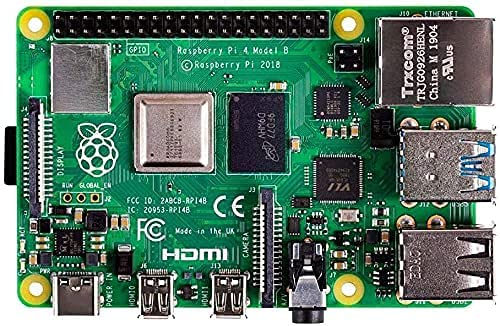
\includegraphics[scale=0.2]{rasp.jpg}
            \caption{Raspberry Pi 4}
        \end{figure}
        
 
        \subsection{Ecran LCD (Raspberry Pi)}
        Un écran LCD de 7 pouces est branché sur le Raspberry Pi et permet d'intéragir avec l'ordinateur.

        \vspace{0.2cm}

        L'intérêt majeur de ce type de périphérique est sa finesse.
        En effet, dans un laboratoire il n’est pas toujours facile d'avoir un grand écran.
        De ce fait avoir un écran de petite taille qu'on peut tenir dans nos mains tout en ayant la possibilité d'utiliser l'écran tactile pour interagir avec l'ordinateur nous permettant de nous dispenser de clavier et de souris.

        \begin{figure}[ht]
            \centering
            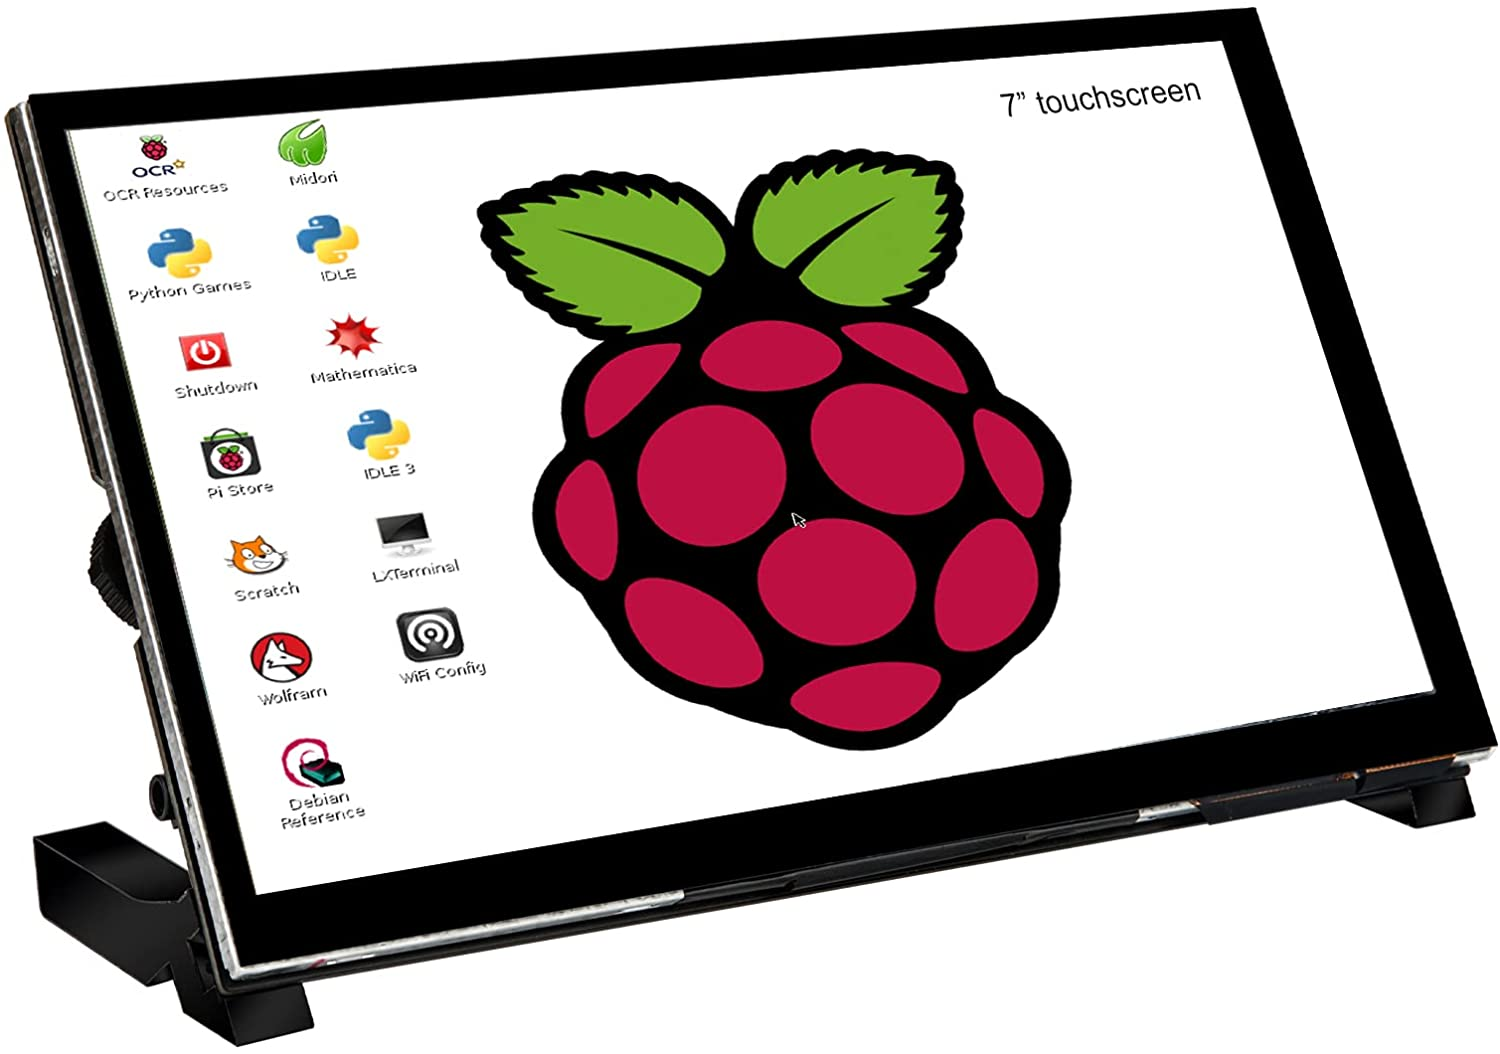
\includegraphics[scale=0.05]{ecran7p.jpg} 
            \caption{Ecran LCD de 7 pouces}
        \end{figure}

        \vspace{1cm}

        \subsection{Module de capture vidéo (Raspberry Pi) V2}
        Le module de capture vidéo (Raspberry Pi) V2 est un module de captation vidéo qui permet de capturer des images et des vidéos.

        % intérêt :
        % - cout, manipulation
        % Inconvénients :
        % - la qualité ?
        % - configuration pas toujours simple - fragile

        \begin{flushleft}
            \begin{itemize}
                \item \textbf{Intérêt :}
                Le principal intérêt de ce module est son coût qui est très faible. De plus tout comme le Raspberry Pi, il est très facile à manipuler. 
                \item \textbf{Inconvénients :}
                la qualité de ce module caméra est relativement mauvaise, sa configuration et son utilisation ne sont pas toujours évidentes.
                De plus il est relativement fragile.
            \end{itemize}                
        \end{flushleft}

        \begin{figure}[ht]
            \centering        
            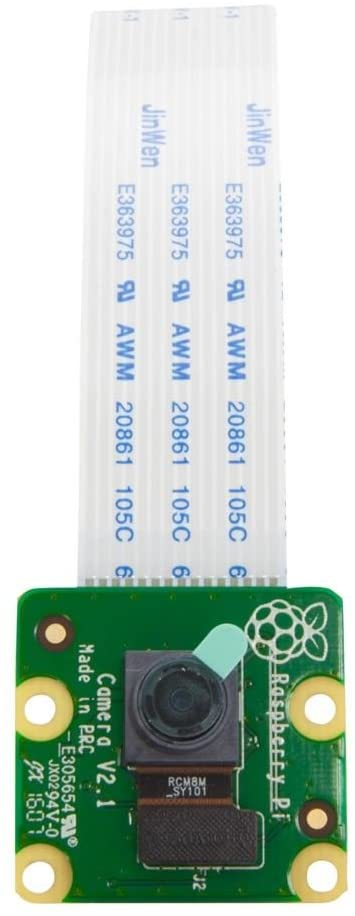
\includegraphics[scale=0.1]{module_cam.jpg}
            \caption{Module de capture vidéo (Raspberry Pi) V2}
        \end{figure}
        
    \section{Montage, Installation et Configuration}
        % du unpack au systeme fonctionnel ... Méthodo, doc , etc ...
        Il faut savoir que le Raspberry Pi et son module caméra arrive séparément ce qui signifie que le module n’est pas monté sur le Raspberry Pi.
        Le Raspberry Pi arrive sans son système d'exploitation préinstallé.
            \subsection{Montage du matériel}
            Le Raspberry Pi possède un port CSI 'Camera Serial Interface' (signifiant en anglais interface série pour caméra, CSI) est un standard d'interface électronique entre une caméra (un capteur ou une source vidéo) et un microprocesseur.

            \begin{figure}[ht]
                \centering
                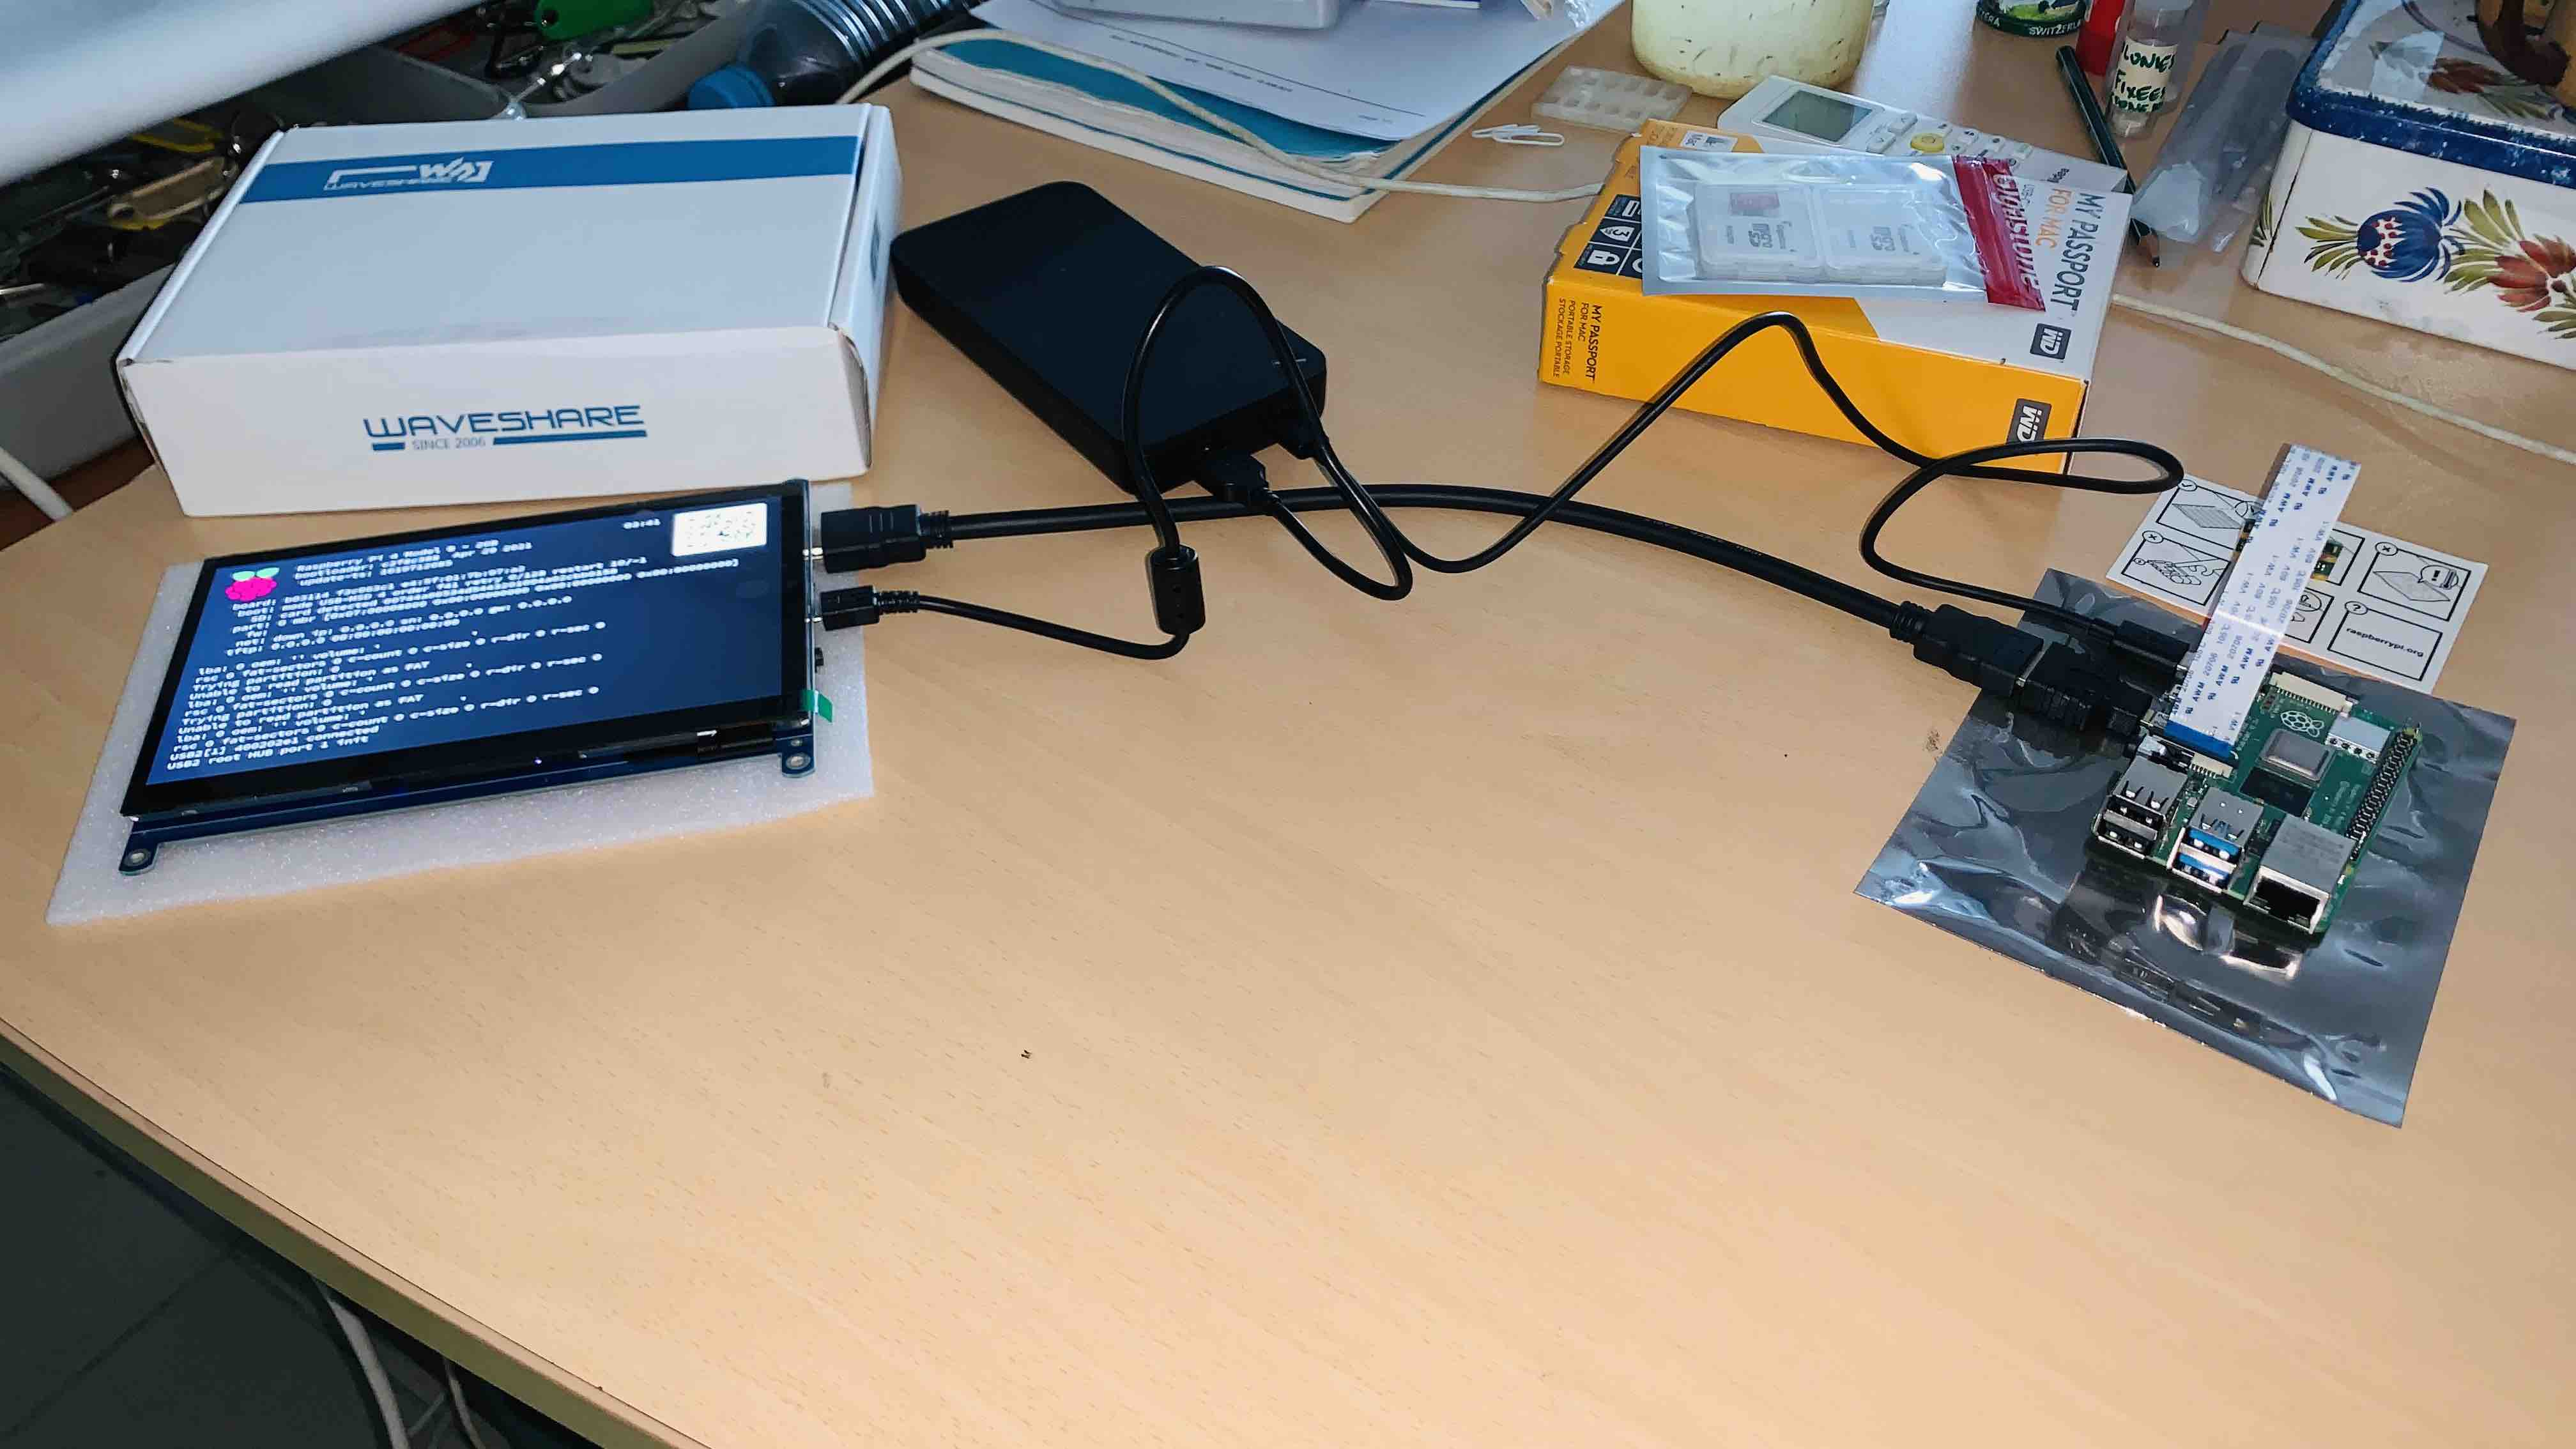
\includegraphics[scale=0.04]{unpack.jpeg} 
                \caption{Matériel assemblé et prêt à l'emploi}
            \end{figure}

            Afin de pouvoir utiliser le module caméra il nous faut donc insérer la nappe de connecteur de la caméra dans le port CSI du Raspberry Pi.
            \subsection{Installation du matériel}
            % Qu'est ce que linux
            Il nous faut installer le système d'exploitation (\underline{$OS^{\ref{def:OS}}$}). Pour ce faire nous allons utiliser Raspberry Pi Imager, logiciel développé par Raspberry Pi Foundation nous permettant de télécharger et installer l'OS \underline{Raspbian}. Raspbian est l'\underline{OS} original ainsi que le plus connu, libre et gratuit basé sur Debian, il est optimisé pour fonctionner sur les différents Raspberry Pi.
            
            \vspace{0.2cm}

            Raspberry Pi Imager est le moyen rapide et facile d’installer Raspberry Pi \underline{OS} (Raspbian) sur une microSD. 

            % Il nous faut télécharger le fichier d'installation sur le site web Raspberry.com et de l'installer.

            \begin{figure}[ht]
                \centering
                \includegraphics[scale=0.3]{Installation_1.png} 
                \caption{Interface "Raspberry Pi Imager"}
            \end{figure}

            Nous obtenons alors l'aperçu de la figure 4.5.
            Comme nous pouvons le voir sur cette figure, le logiciel nous demande de choisir l'OS que nous souhaitons installer.
            On lui indique donc que nous voulons installer l'OS Raspbian en 32 bits. Et on choisit notre stockage qui dans notre cas est une microSD.

            \vspace{0.2cm}

            Une fois cela fait, on lance l'écriture, le logiciel va télécharger l'\underline{OS} et l'installer sur la microSD.

    
            \subsection{Configuration du matériel}
            Avant de pouvoir utiliser le module caméra, activer l'interface caméra.
            Pour ce faire nous allons utiliser la commande \textbf{sudo raspi-config}.

            \begin{figure}[ht]
                \centering
                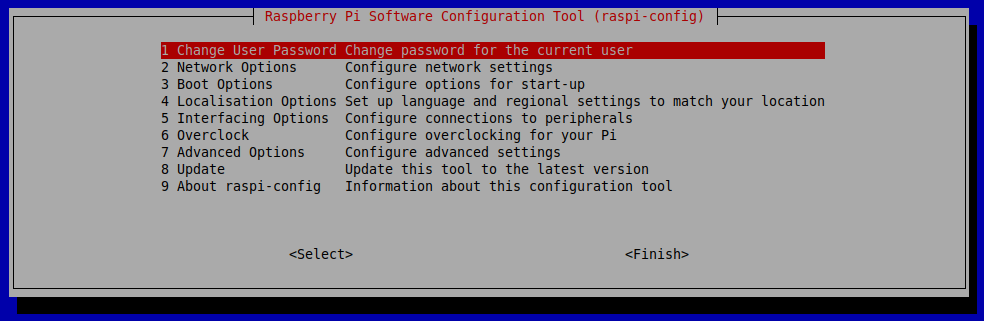
\includegraphics[scale=0.3]{raspi-config.png} 
                \caption{Interface "raspi-config"}
            \end{figure}

            \begin{flushleft}
                
                Une fois dans \textbf{Raspi-config}, nous allons choisir la section \textbf{Interface section}.
            
                \begin{figure}[ht]
                    \centering
                    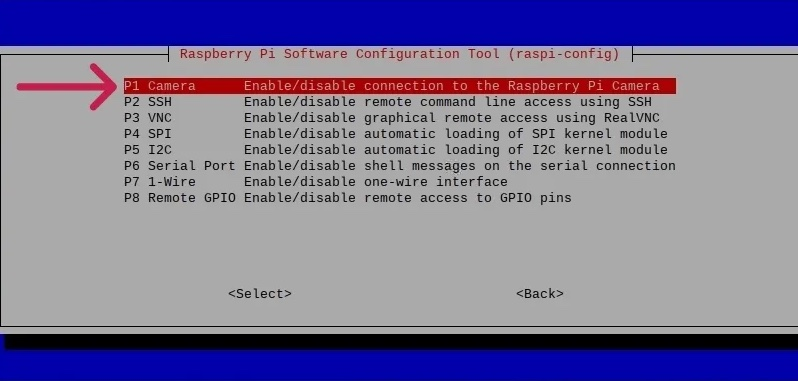
\includegraphics[scale=0.3]{raspiconfig-camera-option.jpg} 
                    \caption{camera option (raspi-config)}
                \end{figure}

                On sélectionne \textbf{P1 Camera} et on met sur \textbf{Enable}.

                \vspace{0.2cm}

                Une fois cela fait on peut quitter \textbf{Raspi-config} et tester si la caméra est bien activée et fonctionne correctement.

                \vspace{0.2cm}

                Pour ce faire, on ouvre le terminal et on tape la commande suivante :

                \begin{flushleft}
                    \begin{lstlisting}[language=bash]
                        raspistill -o Desktop/image.jpg
                    \end{lstlisting}
                \end{flushleft}

                Cette commande nous permet de prendre une photo et de la sauvegarder dans le dossier Desktop. Si photo est bien prise on peut en deduire que la caméra est opérationnelle. 
                
                L'opération suivant consiste à essayer de faire une vidéo.

                \begin{flushleft}
                    \begin{lstlisting}[language=bash]
                        raspivid -o Desktop/video.h264
                    \end{lstlisting}
                \end{flushleft}

                Cette commande nous permet de prendre une vidéo et de la sauvegarder dans le dossier Desktop, la vidéo est bien prise.
                %  Donc tout est fonctionnel.
                
            \end{flushleft}

    \section{Choix des technologies}
        Pour le choix du langage de programmation, Nous nous sommes basé sur les langages de programmation les plus utilisés avec le système d'exploitation \underline{Raspbian}. Lors de ma recherche, 5 langages de programmation sont sortis : 

        \begin{itemize}
            \item Python
            \item C
            \item Java/BlueJ
            \item Perl
            \item Scratch
        \end{itemize}

        Nous constatons que le langage Python est le plus utilisé pour le système d'exploitation Raspbian. Ce qui est normal, car le Pi dans "Raspberry Pi" signifie "Python". Il a donc le mérite d'être le choix par défaut.

        \vspace{0.2cm}

        Afin de pouvoir nous décider sur le langage de programmation, il me faut chercher la compatibilité des \underline{$API^{\ref{def:API}}$} pour la camera. Il s'avère que l'API PiCamera est installée par défaut sur le système d'exploitation Raspbian. Puisque le langage Python et l'API PiCamera sont compatibles, et installé par défaut sur le système d'exploitation Raspbian, il est possible de choisir le langage Python.

        \vspace{0.2cm}
    
        Même si le langage de programmation JavaScript ne figure pas dans cette liste, il est très utilisé, il est donc très intéressant de le choisir.
        Avec electron et nodejs, nous pouvons très bien créer une application multiplateforme. De plus, l'API PiCamera est disponible pour le langage JavaScript.    

        NodeJs et Electron ne sont pas installés par défaut sur le Raspberry Pi, donc cela nous prendra plus de temps afin de réaliser les phases d'installation et de configuration de l'environnement de travail, et plus d'incertitudes qu'avec le langage Python. En vu du délais court, nous allons choisir le langage Python.

        \vspace{0.2cm}
        
        Python est un langage de programmation interprété, multi-paradigme et multiplateformes. Il favorise la programmation impérative structurée, fonctionnelle et orientée objet.
        
        % définir le multi-paradigme
        % définir le multiplateformes
        % Programattion interprété, structurée, fonctionnelle et orientée objet


    % Qu'est ce que le langage Python ?
    
    \section{Réalisation de l'application}
        Avant toutes choses, nous allons importer les modules nécessaires.
        Nous allons utiliser les modules :
        \begin{itemize}
            \item \textbf{picamera :} \textit{Module de la caméra}
            \item \textbf{tkinter :} \textit{Module de l'interface graphique}
            \item \textbf{datetime :} \textit{Module de gestion de la date et de l'heure}
            \item \textbf{os :} \textit{Module de gestion de l'OS}
            \item \textbf{time :} \textit{Module de gestion du temps}
        \end{itemize}

        \vspace{0.2cm}
        
        Nous allons créer une maquette du menu principal de l'application.
        Cette maquette nous permettra d'avoir un aperçu de l'application.
        Et nous permettra de concevoir l'interface graphique (\underline{$GUI^{\ref{def:GUI}}$}) de l'application à l'aide de Tkinter.            

        \subsection{Création de l'interface graphique}
            \begin{figure}[ht]
                \centering
                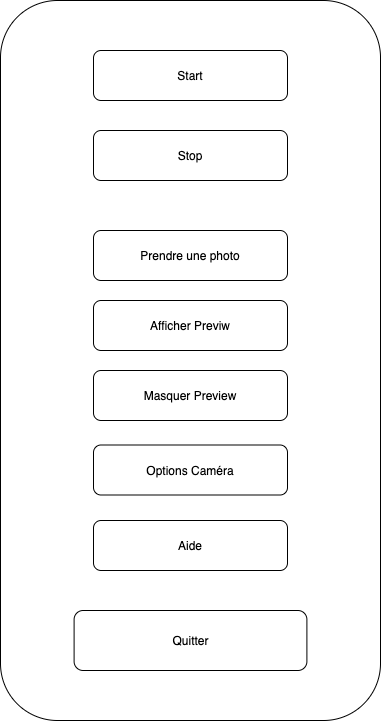
\includegraphics[scale=0.3]{maquette.png} 
                \caption{Maquette de l'application}
            \end{figure}

            \begin{flushleft}
                Nous allons créer 5 classes pour notre GUI qui sont :
                \begin{itemize}
                    \item \textbf{class} \textit{App}
                    \item \textbf{class} \textit{AppPhotoSection}
                    \item \textbf{class} \textit{AppOptionsSection}
                    \item \textbf{class} \textit{AppUtilitySection}
                    \item \textbf{class} \textit{AppHelpSection}
                \end{itemize}                            
            \end{flushleft}

            La classe \textit{App} est la classe principale de notre application.
            C'est ici que nous allons définir la taille de la fenêtre, la couleur de fond, le titre de la fenêtre, le logo de l'application, etc.

            \vspace{0.2cm}

            C'est également dans cette classe que nous allons lancer notre menu principal par la méthode : \textbf{def \_\_init\_\_(self, master)}. La méthode \_\_init\_\_ peut être appelée lorsqu'un objet est créé à partir de la classe, et un accès est nécessaire pour initialiser les attributs de la classe. Le menu principal est représenté par la maquette de la figure 4.8.

            \vspace{0.2cm}

            Les 4 autres class sont les classes qui représentent les sections de l'application.
            Lorsque que l'utilisateur clique sur un des boutons du menu principal, il se rend dans la section correspondante.
        
        \subsection{Fonction Start Recording}
            Afin de réaliser l'application, nous allons commencer par concevoir la fonction cœur de l'application.
            C'est à dire la fonction qui va nous permettre de lancer un enregistrement et de l'arrêter.    
            Cette fonction, son fonctionnement est représenté par la figure 4.9

            \begin{figure}[ht]
                \centering
                \includegraphics[scale=0.4]{diagram_activité_enregistrement.png} 
                \caption{Diagramme d'activité de la fonction "Démarrer un Enregistrement"}
            \end{figure}

            % \newpage
            
            D'après notre diagramme d'activité, il nous faut commencer l'enregistrement lorsque l'utilisateur clique sur le bouton "Start". Avant de pouvoir démarrer un enregistrement, il faut initialiser la caméra, pour cela, la documentation nous indique une fonction qui est : \textbf{camera = PiCamera()}. Une fois la caméra initialisée, nous pouvons commencer à traiter la demande de l'utilisateur.

            \vspace{0.2cm}
            
            \textbf{AskForSaveFile} est une fonction de \textbf{tkinter} qui nous permets de demander à l'utilisateur de saisir un nom de fichier et de lui permettre de choisir l'emplacement de sauvegarde. Une fois que l'utilisateur a saisi le nom de fichier, nous pouvons commencer à enregistrer avec la fonction de l'API PiCamera : \textbf{camera.start\_recording(nomDuFichier, format)}.
            L'enregistrement restera actif tant que l'utilisateur ne clique pas sur le bouton "Stop".
            L'arrêt de l'enregistrement se fait avec la fonction de l'API PiCamera : \textbf{camera.stop\_recording()}.

            \vspace{0.2cm}

            Lors des tests, nous avons remarqué qu'arrêter l'enregistrement de manière manuelle n'est parfois pas très optimale. Dans notre cas, une expérience est d'une durée minimum de 20 minutes, l'utilisateur doit donc rester attentif afin d'arrêter l'enregistrement. Il se peut que l'utilisateur oublie l'enregistrement en cours. 
            
            Nous avons donc décidé de créer une fonction nous permettant de stopper de manière automatique l'enregistrement. Il s'agit de permettre à l'utilisateur de saisir un temps en minutes et de lancer l'enregistrement. Le temps saisi en minute de l'utilisateur sera converti en secondes.

            \vspace{0.2cm}

            De ce fait, l'API PiCamera nous permet de définir le temps d'enregistrement en secondes avec la fonction : \textbf{camera.wait\_recording(tempsEnSeconde)}. Cependant cette fonction possède un défaut, elle agit comme une fonction \textbf{wait()} classique. Par conséquent, durant l'enregistrement, l'utilisateur ne peut pas interagir avec l'application. 
            
            \vspace{0.4cm}

            Une fois que nous n'utilisons plus la caméra, nous pouvons couper toute utilisation de la caméra avec la fonction de l'API PiCamera : \textbf{camera.close()}.
            
        \subsection{Prendre une capture}
        La fonction prendre une capture est une fonction qui va nous permettre de prendre une photo.
        Cette fonction est représenté par la figure 4.10.
        \begin{figure}[ht]
            \centering
            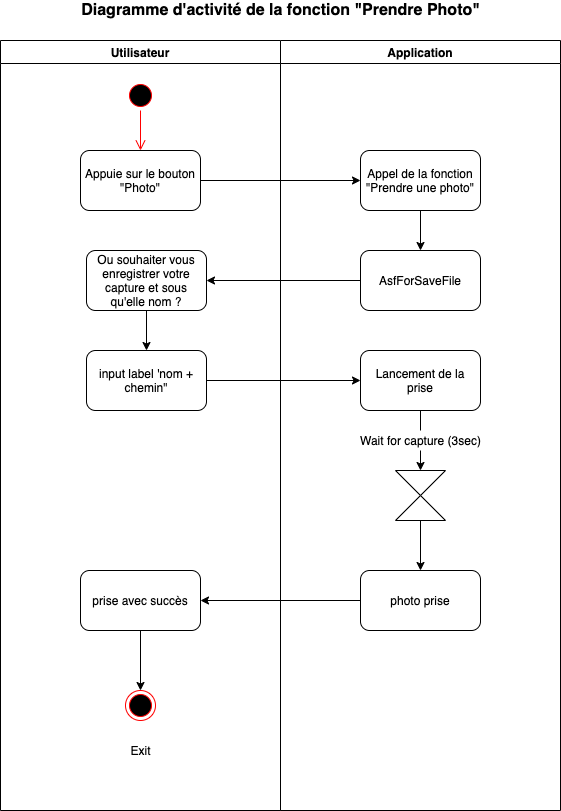
\includegraphics[scale=0.4]{diagram_3.png} 
            \caption{Diagramme d'activité de la fonction "Prendre une capture"}
        \end{figure}

        Contrairement à la fonction \textbf{Démarrer un Enregistrement}, cette fonction est plus simple dans l'ensemble de son fonctionnement. 
        
        \vspace{0.2cm}

        Tout d'abord, comme nous l'avons vu pour la fonction \textbf{Démarrer un Enregistrement}, nous allons initialiser la caméra. Une fois celle-ci initialisée, nous allons demander à l'utilisateur de saisir un nom de fichier et l'emplacement de sauvegarde. Une fois cela fait, il nous faudra préchauffer la caméra afin de pouvoir lancer la capture d'image. Avec la fonction \textbf{sleep()}, nous allons attendre un certain délai avant de lancer la capture.
        Pour le préchauffage, 2-3 secondes suffiront.

        \vspace{0.2cm}

        Une fois cela fait, nous pouvons lancer la capture avec la fonction de l'API \textbf{camera.capture(nomDuFichier, format)}. Nous avons également décidé d'ajouter une fonction permettant de prendre des photos en continu.

        \vspace{0.2cm}

        Nous allons donc créer une fonction permettant de prendre des photos en continu.
        Afin de pouvoir faire cela, nous allons demander à l'utilisateur de saisir un nom de fichier et l'emplacement de sauvegarde comme précédemment.
        Mais avant cela, nous demandons à l'utilisateur de choisir le nombre de photos à prendre.

        \begin{flushleft}
            Pour cela, nous utilisons une boucle telle que : 
            \begin{verbatim}
                for nomDuFichier in camera.record_sequence(
                    '%d.h264' % i for i in range(1, nombreDePhoto)):
                camera.wait_recording(6)
            \end{verbatim}            
        \end{flushleft}

        Tant que le nombre de photos voulues n'est pas atteint, nous allons continuer à prendre des photos toutes les 6 secondes. Nous avons mis un délai de 6 secondes entre chaque photo afin que la prise ne soit pas exactement identique à la précédente.
    
        \subsection{Travail en laboratoire}
        Tout le système que nous avons créé jusqu'à maintenant est destiné à être utilisé dans un laboratoire. De ce fait, le module caméra sera installé sur une potence au-dessus d'un bac ou sera installé diverses espèces lors des expérimentations. Cette installation suit la figure 4.11.

        \begin{figure}[ht]
            \centering
            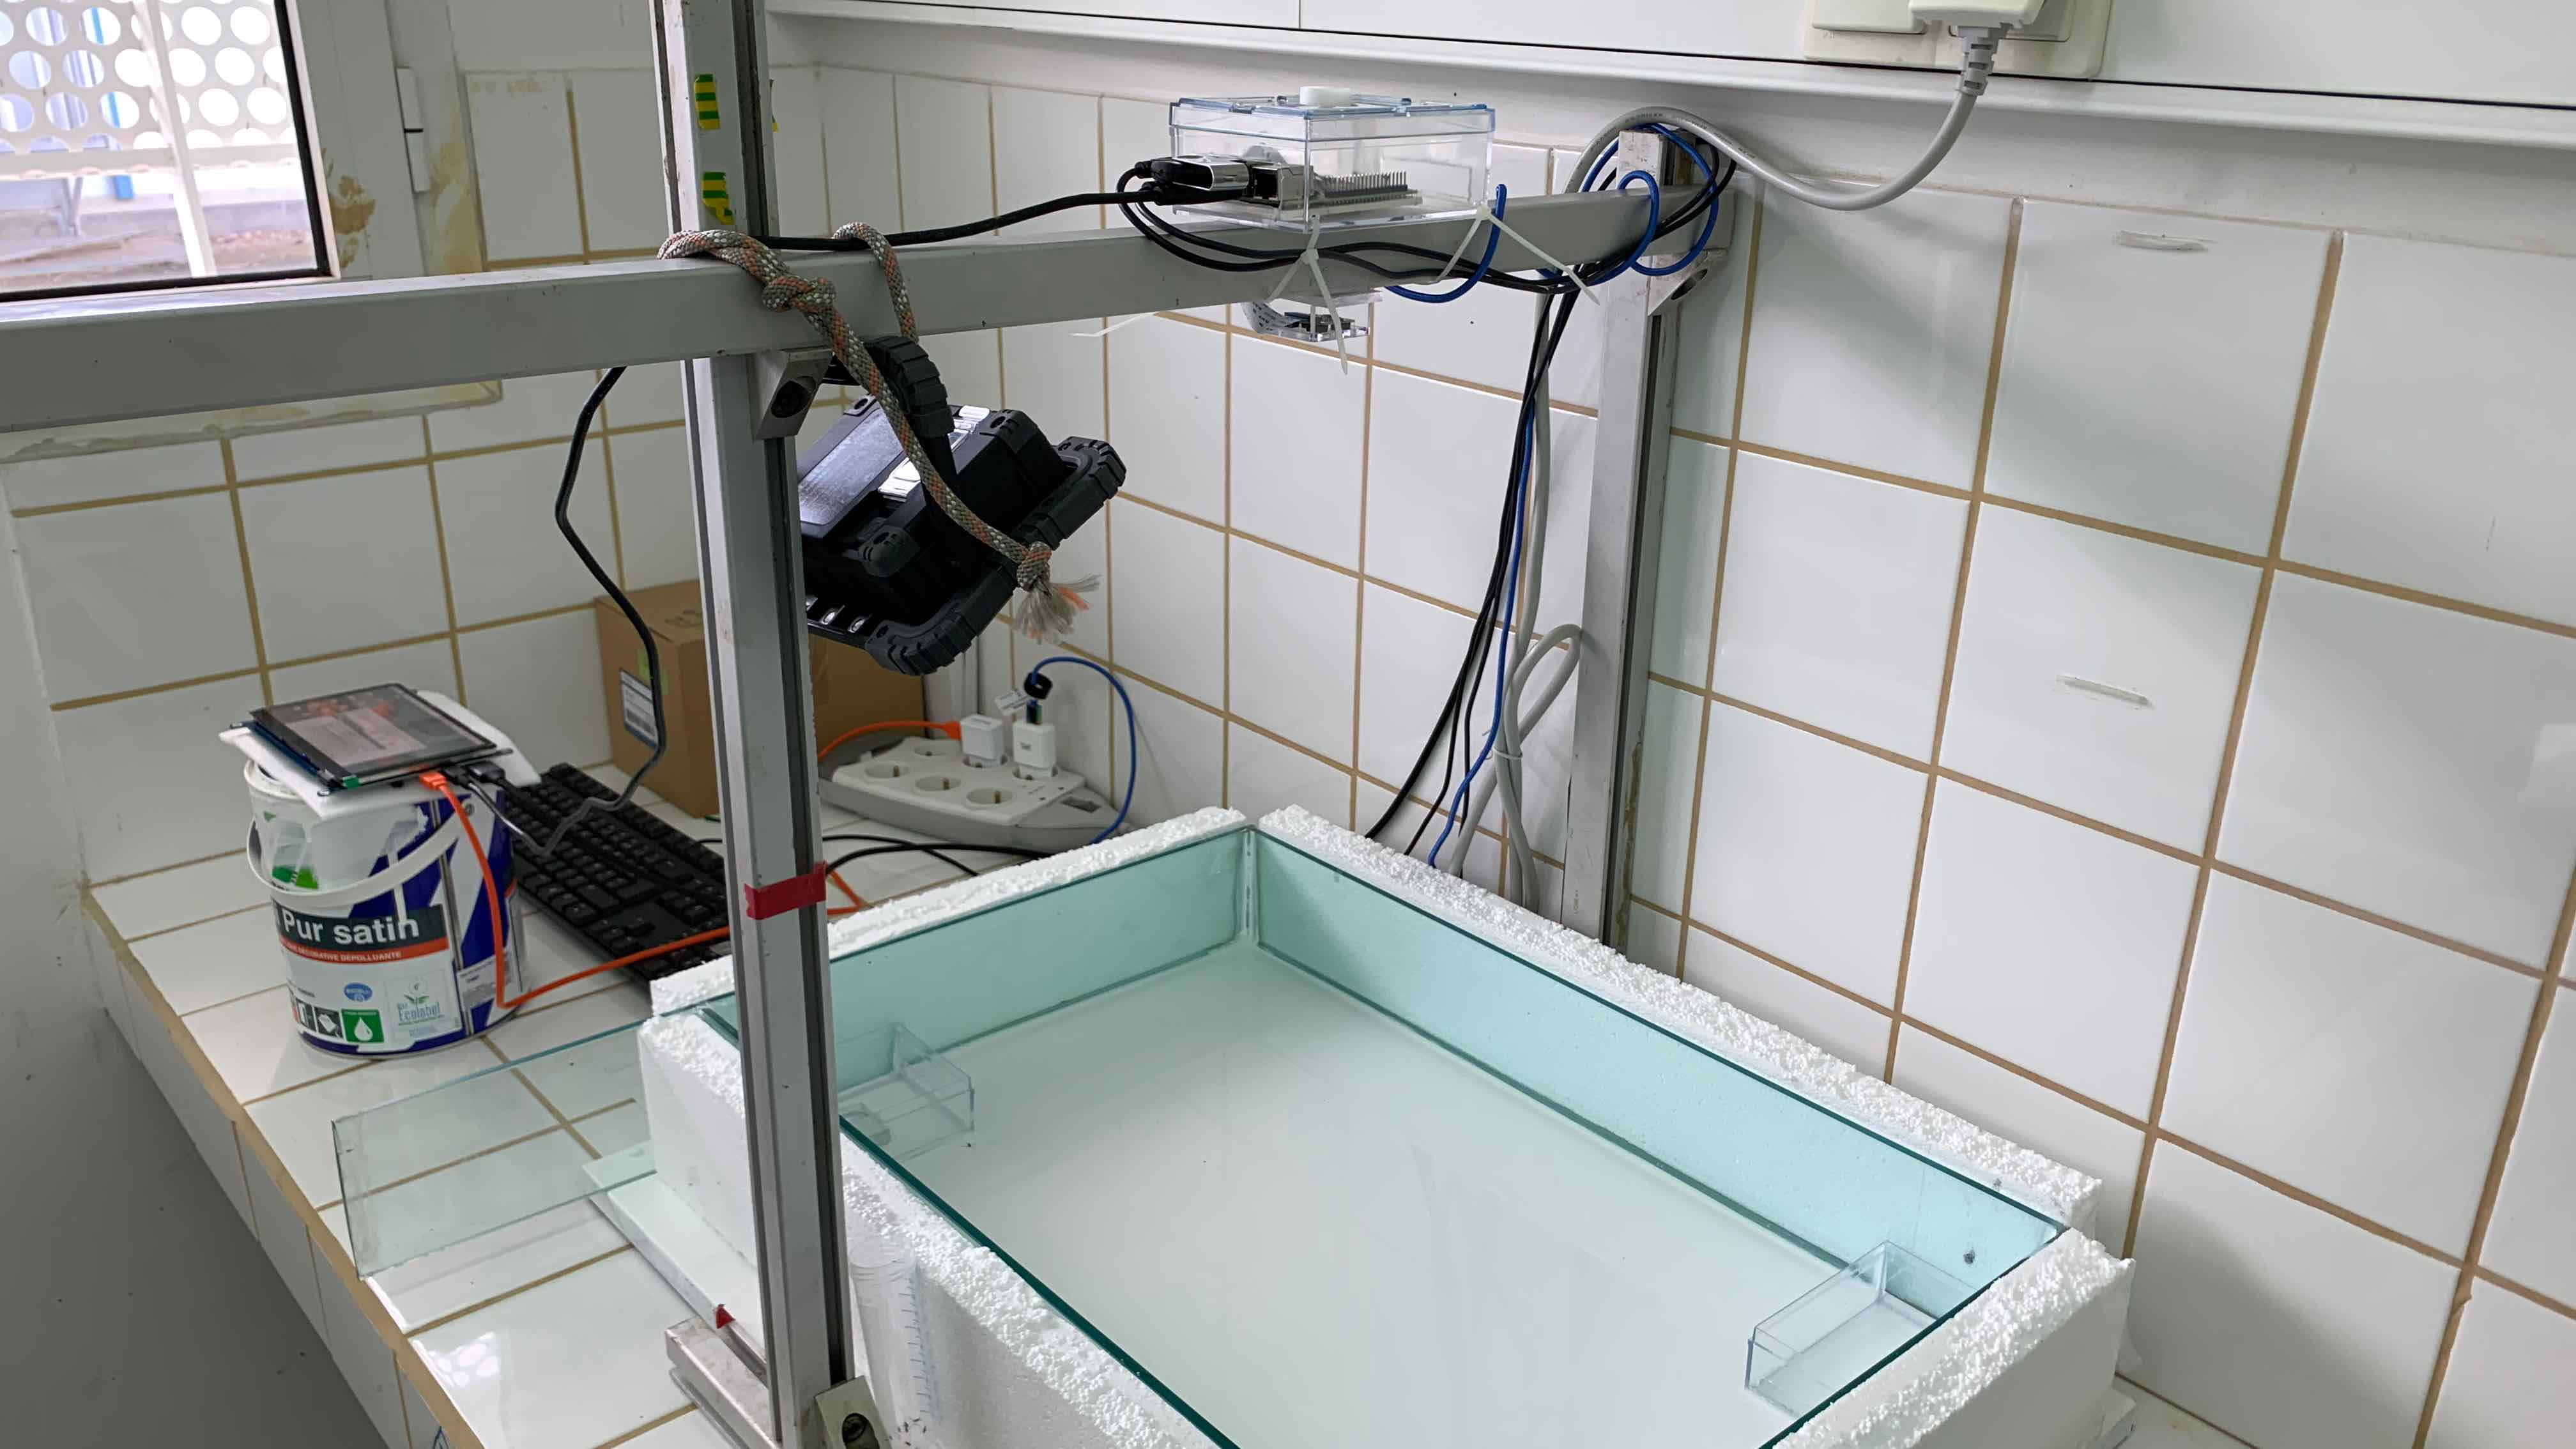
\includegraphics[scale=0.055]{setup.jpeg} 
            \caption{Le dispositif installé dans le laboratoire}
        \end{figure} 

        Nous remarquons que le Raspberry Pi est installé sur une potence dans un boitier afin de le protéger des diverses éclaboussures, il en va de même pour la caméra qui se trouve en bas de la potence. Plus à gauche, nous pouvons voir l'écran tactile qui ne prend pas énormément de place, et qui est relativement amovible.

        \vspace{0.2cm}

        Les \textbf{Gerridés} utilisés pour les expériences sont directement attrapé à l'épuisette dans la Mangrove. Nous avons eu l'occasion de partir à la recherche de ces \textbf{Gerridés} dans la Mangrove de la Guadeloupe (voir Figure 4.12).

        \begin{figure}[ht]
            \centering
            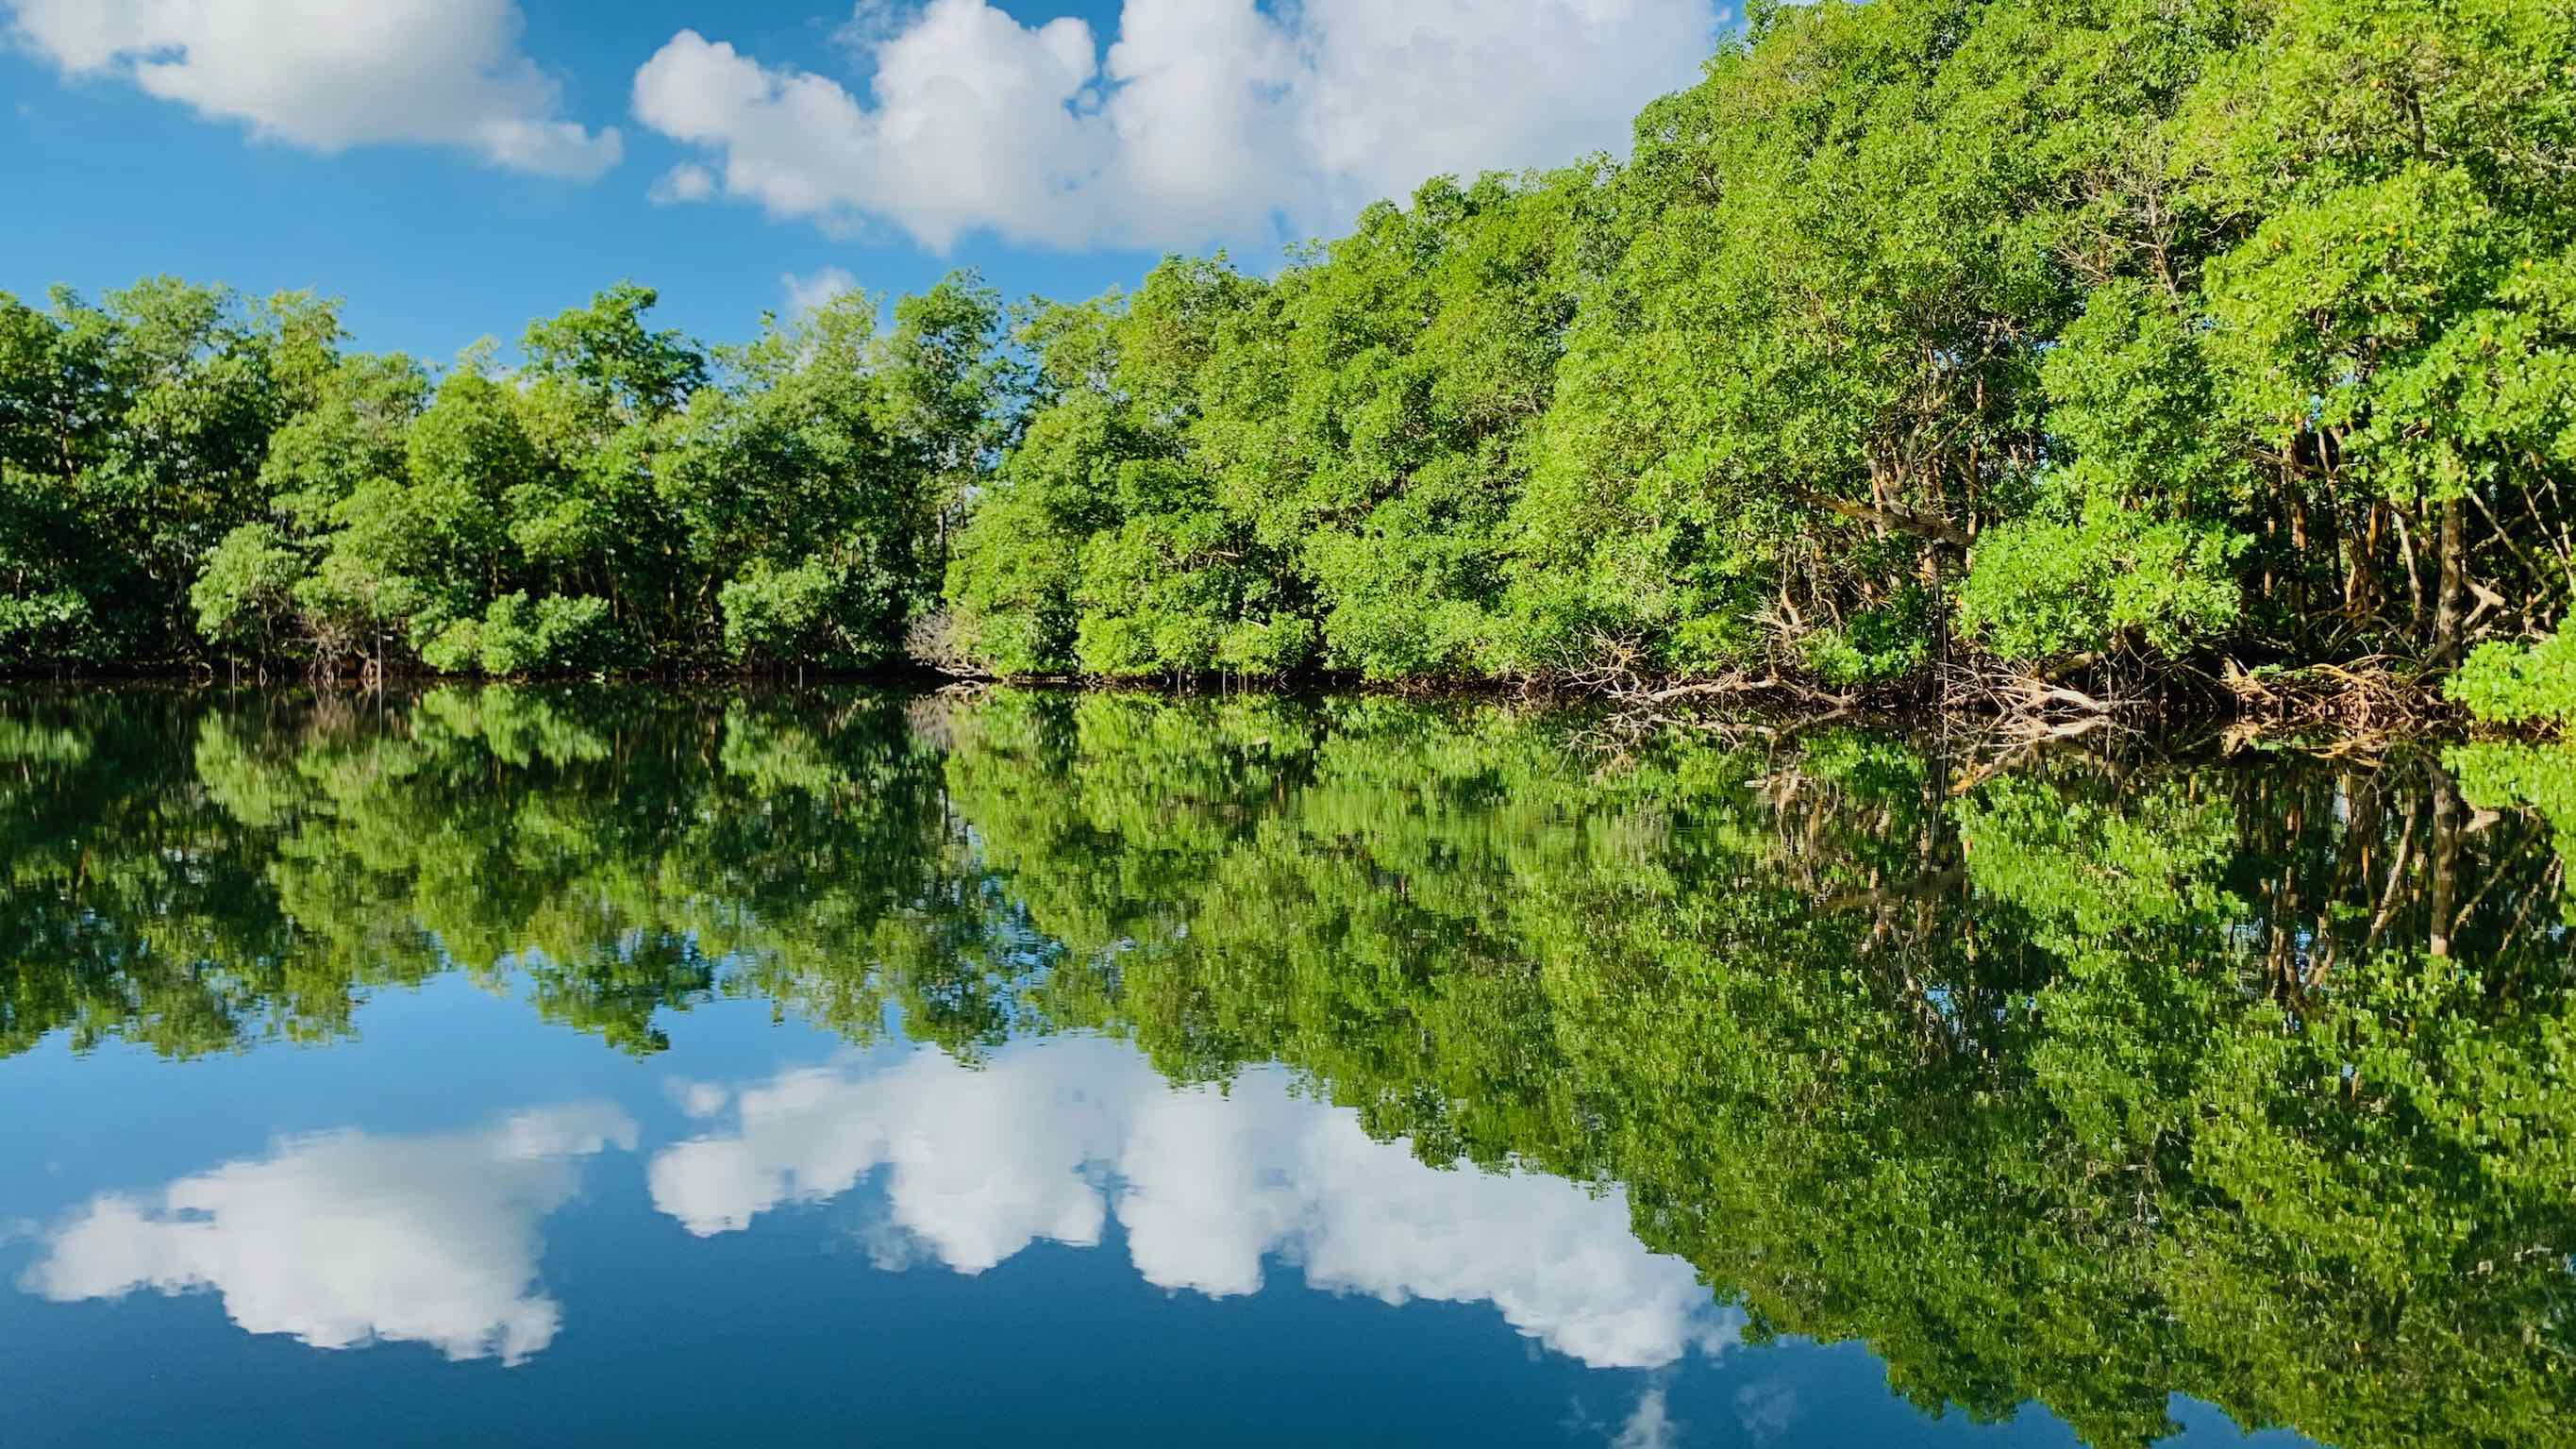
\includegraphics[scale=0.075]{mangrove.jpeg}
            \caption{Mangrove de la Guadeloupe}
        \end{figure}

        \vspace{3.5cm}
             
        \subsection{Travail sur la caméra}
        Le module caméra est très certainement celui qui nous a posé le plus de problème. Pendant une grande partie des expérimentations, nous avons eu divers problèmes lors des enregistrements.

        \vspace{0.2cm}

        Commençons par des problèmes de stockage de la vidéo. Pour nos expérimentations, nous devons réaliser des enregistrements d'une vingtaine de minutes.
        Cela représentait plus de 4Go de mémoire.
        Cela était trop grand pour le stockage de la vidéo sur le Raspberry Pi.

        \vspace{0.2cm}

        Nous avons également eu des soucis d'éclairage, qui provoquaient des effets d'anneaux sur la vidéo, cela a plus ou moins été réglé en modifiant le nombre de données traités par unité de temps (\underline{bitrate}) de l'enregistrement, ainsi qu'en mettant le dispositif dans un endroit sans éclairage.
        L'utilisateur peut également modifier le contraste et la luminosité de la vidéo afin d'avoir un meilleur rendu.

        \vspace{0.2cm}

        % Nous avons rencontré également deux autres problèmes qui sont notamment les effets de zoom lors de nos enregistrements qui étaient dus à une trop forte résolution de la caméra ainsi qu'un problème de saut d'image dans nos enregistrements. Cela étant dû au format de la vidéo, lors de la conversion vidéo en format mp4, ce souci n'apparaissait plus.

        Nous avons également rencontré deux autres problèmes, le premier concernent les effets de zoom lors de nos enregistrements qui étaient dus à une trop forte résolution de la caméra. Le deuxième était un problème de saut d'image dus à un souci au niveau du format de la vidéo.
        Lors de conversion de la vidéo en format mp4, ce dernier problème a été résolu.
        Cela laisse à supposer que l'écriture au format \underline{$H264^{\ref{def:H}}$} n'était pas adapté pour la configuration de notre Raspberry Pi.

        \subsection{Travail sur vidéo}
        % Ajout de la partie mise au point de la vidéo
        Après avoir utilisé notre dispositif lors des expérimentations, les biologistes ont besoin de résultats et pour ce faire nous devons extraire un certain nombre d'images des vidéos, avec le  \underline{$framework^{\ref{def:framework}}$} \textbf{$FFmpeg$}.

        \vspace{0.2cm}

        FFmpeg est un projet de logiciel libre qui produit des bibliothèques et des programmes pour gérer et manipuler des données multimédias. FFmpeg peut gérer l'ensemble du processus de transcodage, de manipulation de vidéos et d'images (redimensionnement, débruitage, etc.), de conditionnement, de diffusion en continu et de lecture. Il s'agit du logiciel de traitement de vidéo et d'image le plus populaire et est utilisé par de nombreuses entreprises dans divers secteurs.

        \begin{flushleft}
            Pour ce faire, nous utilisons une commande de ffmpeg :
        
            \begin{verbatim}
                ffmpeg -i Nom_Vid.h264 -r .6 -q:v 1  ./Nom_Vid_%6d.jpg
            \end{verbatim}            


        \end{flushleft}

        Nous remarquons que cela n'est pas simple d'utiliser cette commande, c'est pourquoi nous avons créé une fonction permettant à l'utilisateur de choisir une vidéo ainsi que le dossier où il souhaite enregistrer les images extraites. 
        
        \vspace{0.2cm}

        Une fois que nous avons nos images, nous pouvons les annoter avec un logiciel en ligne : \textbf{www.robots.ox.ac.uk}.
        Mais le gros problème, c'est qu'il nous faut annoter les images de façon manuelle et une par une, et afin d'avoir des résultats précis, il nous faut travailler avec d'énorme quantité d'image dnas le but d'entrainer un système d'apprentissage automatique, pour un individu annoter environs 900 images n'est pas chose facile.

        \vspace{0.2cm}

        Nous allons donc voir dans la conclusion comment nous améliorer notre système pour que les biologistes puissent travailler avec plus de confort et de rapidité tout en ayant des résultats d'expérimentations de qualité.
 
% Travail réalisé          ===============================

% Conclusion          ===============================
\chapter{Conclusion}
    % (il faut dire à un moment a quoi ca sert tout ça :
    % automatiser la detection des gerridés par traitement des video -> en temps réel !!)
    Ce stage a permis le début du développement d'un système de reconnaissance de Gerridés afin de faciliter le travail des biologistes durant leur expérimentations.
    
    % Finaliser section 1
    % \section{Interface labo / traitement informatique}

    \section{Ressentis par rapport au stage}
    Le travail scientifique que je réalise durant mes études m'a permis de comprendre les différentes documentations allant du montage du Raspberry Pi à la programmation et l'utilisation de l'API PiCamera afin de concevoir l'application. 

    % \begin{flushleft}
        % Nos divers formation en gestion de projet, mon permis de réussir le travail demandé sous contrainte de temps.

        % \vspace{0.2cm}

        % Notre apprentisage universitaire en informatique ma permis de m'adapter rapidement ainsi que de travailler de manière efficace.

        % \vspace{0.2cm}

        % Bien que la formation universitaire permet de bien s'adapter a la vie professionnelle, ce stage en immersion ma permit de dévoiler d'autres facette de mon futur métier. 
    % \end{flushleft}


    \section{Perspectives futures}
    Durant ce stage, nous avons remplacé un dispositif permettant la capture vidéo de qualité en termes de vidéo grâce à la GoPro, mais n'était pas optimisé pour le travail en laboratoire.

    % rappel de la question 

    % humainement ce que j'ai appris 
    % pose la question
    % répodnre la question
    % Limite 

    \vspace{0.2cm}
    
    De ce fait nous avons conçu un dispositif permettant la capture vidéo avec divers fonctionnalités grâce à l'application comme l'arrêt automatique des vidéos, prendre le nombre de photos souhaité en rafale, avec la possibilité d'avoir un rendu de la vidéo en temps réel dans les mains via à l'écran tactile. Bien que nous perdions en qualité d'enregistrement vidéo et photo, nous avons réussi à réaliser un système optimal pour un moindre coût.

    \vspace{0.2cm}

    Mais le système n'est pas fixe, c'est à dire que nous pouvons changer le module caméra par un modèle plus performant afin d'avoir un meilleur rendu vidéo. Concernant l'application, nous pouvons améliorer le fait que l'application se bloque durant le mode rafale ou le mode d'enregistrement automatique en faisant du multiprocessus.
    Cela nous permettrait de réaliser une tâche tout en faisant une autre.

    \vspace{0.2cm}

    Il serait également intéressant d'automatiser l'annotation d'image, en effet annoter une grande quantité d'image est une tâche très longue. Avec la prise de vue en temps réelle, nous pourrions annoter de manière automatique les images et en grande quantité sans que cela soit une tâche fastidieuse.

    


    

% Conclusion          ===============================

% Définition             ===============================

\chapter*{Définition}
    \begin{definition}
        \newcommand{\lab}[1]{(\ref{#1})}

        ARM : ARM est une société britannique spécialisée dans le développement de processeurs d'architecture 32 bits et d'architecture 64 bits de type RISC. Filiale de SoftBank1 depuis 2016. ARM développe également un grand nombre de blocs de propriété intellectuelle (IP). ARM est désormais présent dans le monde entier et son siège historique se situe à Cambridge.

        \label{def:ARM}
    \end{definition}


    \begin{definition}
        \newcommand{\lab}[2]{(\ref{#2})}

        Overclocking : L'overclocking, ou parfois sur-cadencement1, ou surcadençage est une manipulation ayant pour but d'augmenter la fréquence du signal d'horloge d'un processeur au-delà de la fréquence nominale afin d'augmenter les performances de l'ordinateur.

        \label{def:Overclocking}
    \end{definition}

    \begin{definition}
        \newcommand{\lab}[3]{(\ref{#3})}

        OS : Un système d'exploitation (ou système d'exploitation) est un ensemble de programmes et d'outils qui permettent d'exécuter des programmes sur un ordinateur.

        \label{def:OS}
    \end{definition}

    \begin{definition}
        \newcommand{\lab}[4]{(\ref{#4})}

        Paradigme : Un paradigme de programmation est une façon d'approcher la programmation informatique et de traiter les solutions aux problèmes et leur formulation dans un langage de programmation approprié.

        \label{def:Paradigme}
    \end{definition}

    \begin{definition}
        \newcommand{\lab}[5]{(\ref{#5})}

        API : (Application Programming Interface) est une interface de programmation qui permet d'accéder à des fonctionnalités d'un logiciel.

        \label{def:API}
    \end{definition}

    \begin{definition}
        \newcommand{\lab}[6]{(\ref{#6})}

        GUI : (Graphical User Interface) est une interface utilisateur graphique qui permet d'interagir avec un logiciel.

        \label{def:GUI}
    \end{definition}

    \begin{definition}
        \newcommand{\lab}[7]{(\ref{#7})}

        H264 : H264 est un codec compressé de type video qui permet de compresser des images en une seule image.

        \label{def:H}
    \end{definition}

    \begin{definition}
        \newcommand{\lab}[8]{(\ref{#8})}

        framework : Un framework est un ensemble de composants qui sont utilisés pour construire un logiciel.

        \label{def:framework}
    \end{definition}


% \makeglossaries

% \newglossaryentry{latex}
% {
%     name=latex,
%     description={Is a markup language specially suited 
%     for scientific documents}
% }

% \newglossaryentry{maths}
% {
%     name=mathematics,
%     description={Mathematics is what mathematicians do}
% }

% Définition             ===============================

% bibliography            ===============================
\begin{thebibliography}{9}
    \bibitem{installation}
    \textbf{Installation du Raspberry Pi}
    \begin{itemize}
        \item \footnotesize{\url{https://www.raspberrypi.com/documentation/computers/getting-started.html}}
        \item \footnotesize{\url{https://www.raspberrypi-france.fr/guide/installer-raspbian-raspberry-pi/}}
    \end{itemize}

    \bibitem{module camera}
    \textbf{Premiers pas avec le module caméra}
    \begin{itemize}
        \item \footnotesize{\url{https://projects.raspberrypi.org/en/projects/getting-started-with-picamera/0}}
    \end{itemize}

    \bibitem{configuration}
    \textbf{Configuration du Raspberry Pi}
    \begin{itemize}
        \item \footnotesize{\url{https://projects.raspberrypi.org/en/projects/raspberry-pi-using/9}}
        \item \footnotesize{\url{https://www.raspberrypi-france.fr/guide/configurer-raspbian/}}
        \item \footnotesize{\url{https://www.raspberrypi-france.fr/guide/connecter-ssh-raspbian/}}
        \item \footnotesize{\url{https://www.waveshare.com/wiki/7HP-CAPQLED}}
    \end{itemize}    

    \bibitem{outils dev}
    \textbf{Documentation API et librairies}
    \begin{itemize}
        \item \footnotesize{\url{https://picamera.readthedocs.io/en/release-1.13/}}
        \item \footnotesize{\url{https://www.npmjs.com/package/pi-camera}}
        \item \footnotesize{\url{https://developer.mozilla.org/en-US/docs/Web/API/File_System_Access_API}}
        \item \footnotesize{\url{https://docs.python.org/fr/3/library/tk.html}}
        \item \footnotesize{\url{https://realpython.com/python-gui-tkinter/}}
    \end{itemize}

    \bibitem{Knowledge resources}
    \textbf{Resources Informative}
    \begin{itemize}
        \item \footnotesize{\url{https://wethegeek.com/programming-languages-for-raspberry-pi/}}
    \end{itemize}
    
\end{thebibliography}
% bibliography            ===============================

\end{document}